% 论文_问题二前两部分.tex —— 问题二前两部分(日内销售结构模型 + 七日需求预测)
% 本文件是章节片段(无 documentclass),预览请打开 论文预览.tex 编译;
% 并入主文档时作为 \input 载入,章节编号自动顺延。
% 与主文档合并时:将本文件作为 \input 载入,章节编号自动顺延;
% 图件 paper_fig1~fig5.pdf 与本文件同目录,需 \graphicspath{{p2/}} 或同目录编译。
% 编译前须填两处表格数据(搜索 %%FILL%%)。 这个词，A检查都。
\section{问题二模型的建立与求解}

本节先刻画六品类蔬菜的日内销售结构,建立"正价、品相折扣、清仓"三渠道的销售模型,说明损耗率与折扣渠道的关系;再在日度尺度上建立七日需求量预测模型。前者给出各渠道的销量占比与实现价格,后者的需求口径与清仓回收价格均取自前者。

\subsection{模型假设}

\begin{enumerate}
  \item \textbf{当日售罄假设}:蔬菜类商品当日进货、当日售完,隔日无法再售。因此各日补货决策相互独立,不存在跨期库存结转。
  \item \textbf{折扣档位假设}:折扣销售存在两个稳定档位,19 时前为品相折扣档(折后价约为原价的 0.80~0.91),19 时起为清仓档(多数品类折后价为原价的 0.600);茄类例外,全天约 0.83 档。渠道归属一律以 19 时为界。
  \item \textbf{损耗口径假设}:附件 4 的损耗率 $\theta$ 为近期盘点口径,刻画进货与陈列中的商品损耗;按题面机制,运损与品相变差的商品通常经折扣渠道售出,故损耗商品与折扣渠道相对应。$\theta$ 同时用作补货换算参数,即补货总量 $=$ 需求$/ (1-\theta)$。
  \item \textbf{需求口径假设}:品类日需求量取正价、品相折扣、清仓三渠道销量合计。疑似提前售罄日的观测销量只构成需求的下界,训练与评价中按删失数据处理。
  \item \textbf{日历假设}:节假日效应以春节、国庆、五一的法定假期窗口哑变量刻画;星期效应用星期哑变量与周季节分解刻画。不考虑天气、客流量、竞争价格等附件未提供的外生变量,其影响并入残差,由分位数区间覆盖。
\end{enumerate}

其中假设 3 与假设 4 需要说明设计理由。假设 3 将损耗率与折扣渠道对应起来:一是承接题面"对运损和品相变差的商品通常进行打折销售"的机制,使折扣渠道的构成有明确的物理含义;二是使收益核算互洽,折扣渠道进入收入端、$\theta$ 进入补货的成本端,若两者脱钩,收益模型会同时漏掉损耗成本与折扣收入。需要说明的是,附件 4 的 $\theta$ 为近期盘点口径,与附件 2 三年流水的统计窗口不同,本文据此将 $\theta$ 用作渠道机制与补货换算的参数,折扣渠道的日内与品类结构由附件 2 实测给出。假设 4 若不成立,即把售罄日的低销量当作真实需求,滞后特征将被系统性污染:例如某日 15 时即售罄、记录销量 120 kg,而真实需求约 150 kg,模型会把该日当低需求日学习,进而低估未来一周的需求。假设 4 的具体处理见 \ref{subsec:censor}。

\subsection{日内销售结构模型}

\subsubsection{渠道划分与损耗率的关系}

对 2020 年 7 月 1 日至 2023 年 6 月 30 日共 878{,}042 条销售流水(已剔除退货),按"时段$\times$是否打折"把每条记录划入三个渠道:不打折记为正价渠道;19 时前打折记为品相折扣渠道,对应题面所述运损与品相受损但仍可售的商品;19 时起打折记为清仓渠道,对应日终未售完商品的降价出清。这样划分的依据是折扣深度的时间结构:全部品类 19 时前的折后价位于原价的 0.80~0.91 档,19 时后多数品类精确落在 0.600 档,呈两档式政策结构,而非随时间连续衰减,故以 19 时为界切分。

在该口径下,损耗率 $\theta$ 与品相折扣渠道相对应:运损与品相变差的商品经折扣渠道变现,清仓渠道则承接当日未售完的部分。表 \ref{tab:theta} 列出各品类的近期损耗率,它在后文的收益模型中进入补货成本端,即补货总量 $=$ 需求$/ (1-\theta)$。

\begin{table}[htbp]
  \centering
  \caption{各品类近期损耗率 $\theta$(附件 4)}
  \label{tab:theta}
  \begin{tabular}{lcccccc}
    \toprule
    品类 & 花叶类 & 食用菌 & 辣椒类 & 水生根茎类 & 茄类 & 花菜类 \\
    \midrule
    $\theta$/\% & 12.83 & 9.45 & 9.24 & 13.65 & 6.68 & 15.51 \\
    \bottomrule
  \end{tabular}
\end{table}

\subsubsection{日内销量分布与渠道结构}

图 \ref{fig:intraday} 给出水生根茎类的日内销量结构(占该品类全期销量的百分比)。销量呈三段式:9 至 10 时为开店高峰,16 至 18 时为次高峰,19 时起进入清仓时段。单小时峰值出现在 10 时,约 18\%;清仓渠道的销量集中在 19 至 21 时,品相折扣则零散分布在 9 至 18 时之间。

\begin{figure}[htbp]
  \centering
  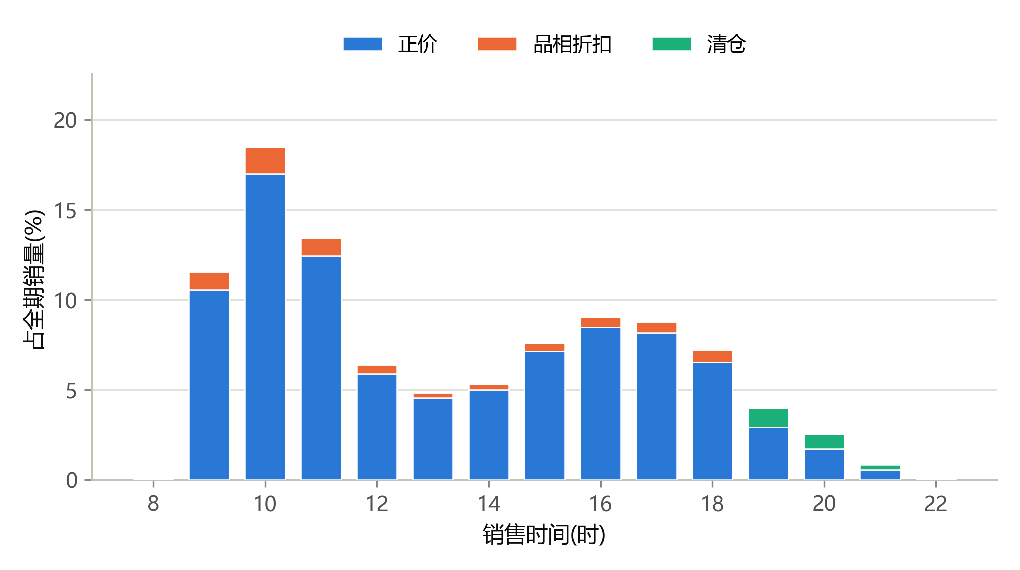
\includegraphics[width=0.92\textwidth]{paper_fig1.pdf}
  \caption{水生根茎类日内销量结构(占全期销量比重/\%,按渠道堆叠)}
  \label{fig:intraday}
\end{figure}

图 \ref{fig:channel} 汇总六品类的渠道构成。正价渠道占各品类销量的 91.0\%~97.3\%,是绝对主体。品相折扣渠道的占比存在品类差异:水生根茎类最高,为 6.9\%,花叶类与茄类最低,约 2.0\%。清仓渠道的占比同样分化:食用菌为 5.4\%、花叶类为 4.7\%,而茄类仅 0.68\%。以清仓与品相折扣的销量之比衡量两类渠道的相对强度,花叶类为 2.35、食用菌为 1.88,呈清仓主导型;水生根茎类为 0.31、茄类为 0.34,呈品相主导型。这一差异与其货架期和损耗特性一致:叶菜类当日未售出的余量大、清仓需求强,茄类耐存放、折扣以挑拣产生的品相损失为主。

\begin{figure}[htbp]
  \centering
  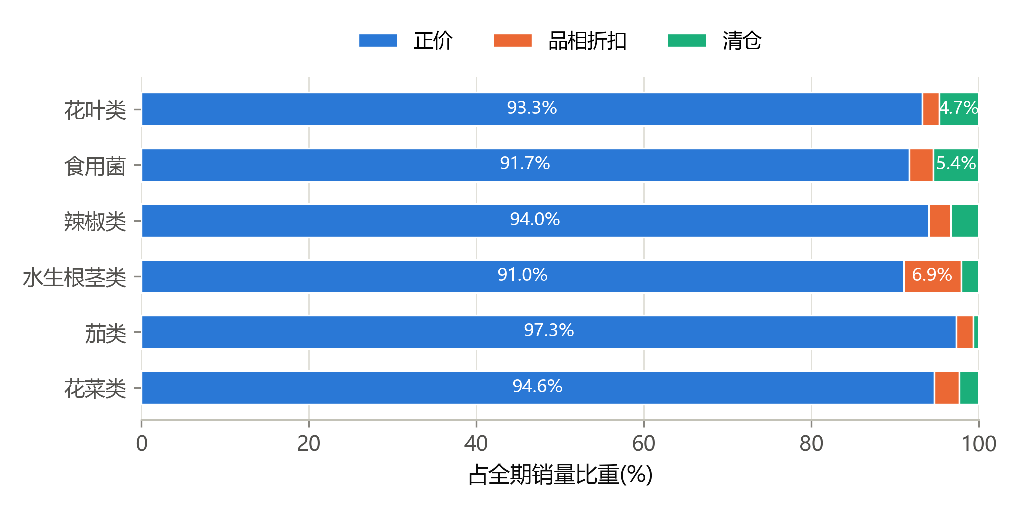
\includegraphics[width=0.92\textwidth]{paper_fig2.pdf}
  \caption{六品类渠道结构(占全期销量比重/\%)}
  \label{fig:channel}
\end{figure}

\subsubsection{折扣深度的时间结构}

图 \ref{fig:depth} 给出花叶类打折记录的折后价与原价之比(中位)随小时的变化。日间该比值从 9 时的 0.81 单调降至 18 时的 0.69,反映商品随陈列时间增加而品相变差、折价逐步加深;19 时起跳变至 0.600 档并保持稳定,对应定时清仓政策。这条曲线同时给出了分时段定价所需的折扣深度函数,也是 19 时渠道划分依据的直接证据。

\begin{figure}[htbp]
  \centering
  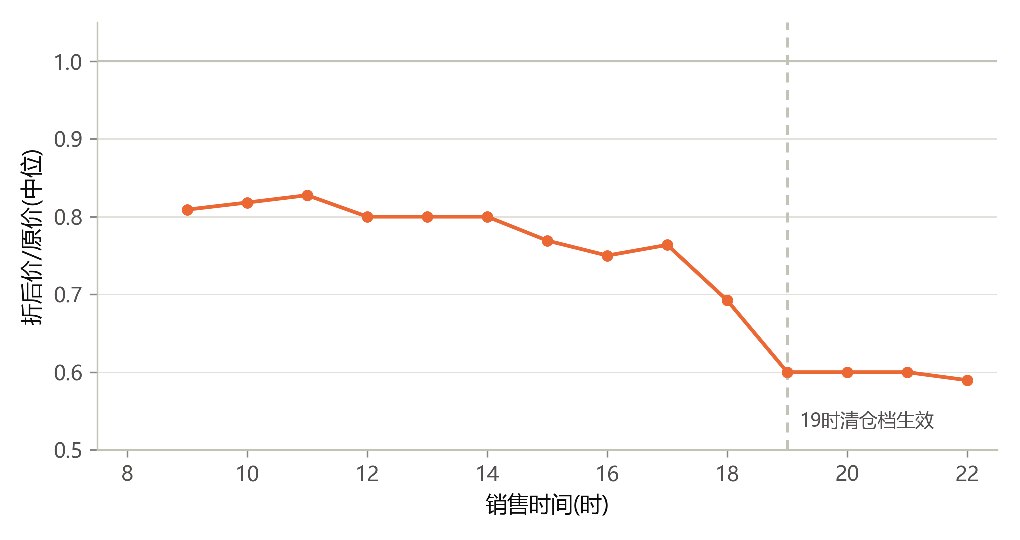
\includegraphics[width=0.92\textwidth]{paper_fig3.pdf}
  \caption{花叶类日内折扣深度曲线(折后价/原价中位,1.0 为原价)}
  \label{fig:depth}
\end{figure}

\subsection{基于周季节分解与 LightGBM 分位数回归的七日需求预测}

\subsubsection{建模思路}

需求预测有三件事要先界定,即预测对象、周季节与节假日的剥离方式,以及销量不等于需求时的处理。本文的口径是:品类日需求量取三渠道销量合计,与补货总量的口径一致;周季节由经典加法分解剥离,节假日与月份作为特征交由模型学习;销量对需求的截断通过一个数据驱动的售罄检测器显式处理,这是本模型与常规做法的主要差别。

\subsubsection{周季节分解}

设品类日销量为 $Q_t$,取 $y_t=\ln(Q_t+0.1)$ 进入模型。周季节采用经典加法分解:
\begin{equation}
  y_t = T_t + S_{w(t)} + \varepsilon_t,
\end{equation}
其中 $T_t$ 为 7 日滑动平均趋势项,$w(t)$ 为 $t$ 日的星期序号,季节因子
\begin{equation}
  S_w = \operatorname*{median}_{t:\,w(t)=w,\,Q_t>0}\,\left(y_t - T_t\right),
\end{equation}
模型在去季节序列 $\tilde{y}_t = y_t - S_{w(t)}$ 上训练,预测时加回 $S_{w(t)}$。分解所需统计量只在各折训练窗内估计;训练窗最后 3 天的趋势项强制用 trailing 窗口计算,避免居中窗口引用未来数据。

\subsubsection{提前售罄检测与删失处理}
\label{subsec:censor}

销量是需求被库存截断后的实现值,售罄日的观测销量低估真实需求,而附件并未提供缺货记录。为此我们构造了一个只依赖销售流水的提前售罄检测器:记品类第 $t$ 日最后一次成交时刻为 $L_t$(时),若
\begin{equation}
  L_t \le \operatorname*{median}\left\{L_{s}:\, s \text{ 为 } t \text{ 前 8 个同星期日}\right\} - 3
  \quad\text{且}\quad
  Q_t \ge \tfrac{1}{2}\,\operatorname*{median}\{Q_{t-28},\dots,Q_{t-1}\},
  \label{eq:censor}
\end{equation}
则将第 $t$ 日标记为疑似提前售罄日。其含义是:营业时长与近期同星期几基本一致,打烊时刻却大幅提前且销量并不偏低,说穿了,就是下午把货卖空了。全部 6 品类 6570 个品类日中共检出 62 天,占比 0.9\%,其中水生根茎类 23 天、茄类 22 天、花菜类 14 天、食用菌 3 天,花叶类与辣椒类为 0 天;检出集中于销量小、波动大的品类,与其断货机理相符。

检测结果在模型中有三处用途。其一,作为特征:售罄标记的滞后值(滞后 7 天与近 7 天检出频率)进入特征矩阵,使模型得以甄别滞后项中被截断的低值。其二,作为训练样本处理:保守方案将标记日从训练中剔除,不以其有偏观测参与拟合;进一步地,利用任务一日内销售结构模型给出的累计销量曲线,把截断日的观测销量按其打烊时刻放大到全天水平,作为需求估计参与训练,记为修复方案。其三,作为评价口径:回测指标分全样本与剔除疑似售罄日两套报告。三种处理连同不作处理的对照一起,由 \ref{subsec:bt} 的消融实验择优。

\subsubsection{LightGBM 分位数回归与直接多步设计}

六个品类共 6570 个日度观测合并为一个训练集,品类以哑变量进入。模型为 LightGBM 分位数回归,目标取 $\alpha=0.1,0.5,0.9$ 三个分位数的分位损失,树数 400、学习率 0.05、叶子数 31、叶最小样本数 30,其余取默认值。这一选型有方法学与领域文献的双重支撑。方法上,梯度提升树自 Ke 等提出 LightGBM 以来\cite{ke2017},凭对非线性关系与特征交互的高效刻画成为表格型预测数据的主力;Grinsztajn 等在中等规模表格数据集上的系统比较进一步表明,树模型的整体表现仍优于深度网络\cite{grinsztajn2022}。领域上,零售需求预测的近期文献结论一致:Lyulyov 对某连锁超市 13 种预测方法的比较中,调参后的 LightGBM 取得最低误差\cite{lyulyov2024};Fan 等针对生鲜品类快速响应供应链构建的 LightGBM 混合模型,也报告了优于对照方法的预测精度\cite{fan2024}。相比之下,单序列深度模型在中小规模序列上并无稳定的优势证据,故本文不引入此类模型。目标变量为去季节后的 $\tilde{y}_t$,预测值经 $\hat{Q}_\alpha=\exp(\hat{q}_\alpha)-0.1$ 换算回千克;由于单调变换保持分位数,该换算是精确的,且保证预测非负。

特征共 37 维,分四组。滞后组是 $\tilde{y}$ 的 7、14、21、28 日滞后及其平移 7 日的 28 日滚动均值与标准差,断货组是式 (\ref{eq:censor}) 标记的滞后值,日历组含星期、月份、年份哑变量与节假日标记,品类组为品类哑变量。滞后项全部取 7 天及更早,单个模型因而能直接输出未来 7 天的预测,不依赖递归调用,避免多步递归的误差累积。

\subsubsection{基线模型与回测方案}
\label{subsec:bt}

设两条基线。季节朴素基线取 $\hat{Q}_t = Q_{t-7}$,即直接以上周同日销量作为预测,它是时序预测的标准下界参照。统计基线取岭回归,与主模型共用同一套周季节分解和特征矩阵,只在模型层以线性回归替代梯度提升树,用以分离特征工程与非线性模型各自的贡献。

回测采用滚动起点方案:以 2023 年 1 月 2 日起每周一个起点,共 24 折,每折以起点前全部数据训练、预测其后 7 天,覆盖 2023 年上半年。评价指标中,加权绝对百分比误差
\begin{equation}
  \mathrm{WAPE}=\frac{\sum_t \left|Q_t-\hat{Q}_t\right|}{\sum_t Q_t},
\end{equation}
直接给出相对总量的误差水平;MASE 与 RMSSE 分别以训练窗内季节差分的平均绝对值和均方根为标尺,
\begin{equation}
  \mathrm{MASE}=\frac{\operatorname*{mean}\left|Q_t-\hat{Q}_t\right|}
  {\operatorname*{mean}\left|Q_t-Q_{t-7}\right|},
  \qquad
  \mathrm{RMSSE}=\frac{\sqrt{\operatorname*{mean}\left(Q_t-\hat{Q}_t\right)^2}}
  {\sqrt{\operatorname*{mean}\left(Q_t-Q_{t-7}\right)^2}},
\end{equation}
两者小于 1 即优于季节朴素基线;分位数质量以 pinball 损失评价,
\begin{equation}
  L_\alpha(y,\hat{q})=\operatorname*{mean}\left[\alpha\,(y-\hat{q})\,\mathbf{1}_{y\ge\hat{q}}+(1-\alpha)\,(\hat{q}-y)\,\mathbf{1}_{y<\hat{q}}\right].
\end{equation}

\begin{table}[htbp]
  \centering
  \caption{回测指标对照(2023 年 24 折滚动平均)}
  \label{tab:bt}
  \begin{tabular}{lcccccc}
    \toprule
    模型 & WAPE & MASE & RMSSE & pinball10 & pinball50 & pinball90 \\
    \midrule
    STL+LightGBM(断货修复) & 0.2406 & 0.730 & 0.516 & 3.95 & 9.18 & 6.55 \\
    STL+LightGBM(断货剔除) & 0.2440 & 0.734 & 0.520 & 3.92 & 9.17 & 6.64 \\
    STL+LightGBM(无断货处理) & 0.2447 & 0.741 & 0.525 & 3.95 & 9.33 & 6.47 \\
    STL+岭回归 & 0.2874 & 0.834 & 0.580 & -- & -- & -- \\
    季节朴素 & 0.3060 & 0.929 & 0.660 & -- & -- & -- \\
    \bottomrule
  \end{tabular}
\end{table}

表 \ref{tab:bt} 与图 \ref{fig:wape} 给出回测结果。主模型 STL+LightGBM(断货修复)的整体 WAPE 为 0.2406,比不作断货处理的同型模型降低 1.7\%,比岭回归基线降低 16.3\%,比季节朴素基线降低 21.4\%;MASE 为 0.730,小于 1,7 天预测误差较"照抄上周同日"低 27.0\%。消融实验中两档断货处理均优于不作处理,且修复档最优,说明任务一的日内结构不仅刻画了销售形态,其累计销量曲线反哺训练目标后还带来了额外收益。分品类来看,修复档在六个品类全部持平或占优,改善最大的为茄类(WAPE 由 0.288 降至 0.281)与花叶类、食用菌(约降 2.6\%);花叶类与辣椒类全期未检出售罄日,各档结果几乎重合,说明该处理不引入副作用。图 \ref{fig:wape} 左下还显示,主模型在全部六个品类上的 WAPE 均低于两条基线,误差最大的为水生根茎类(0.295),最小的为花叶类(0.180)。

\begin{figure}[H]
  \centering
  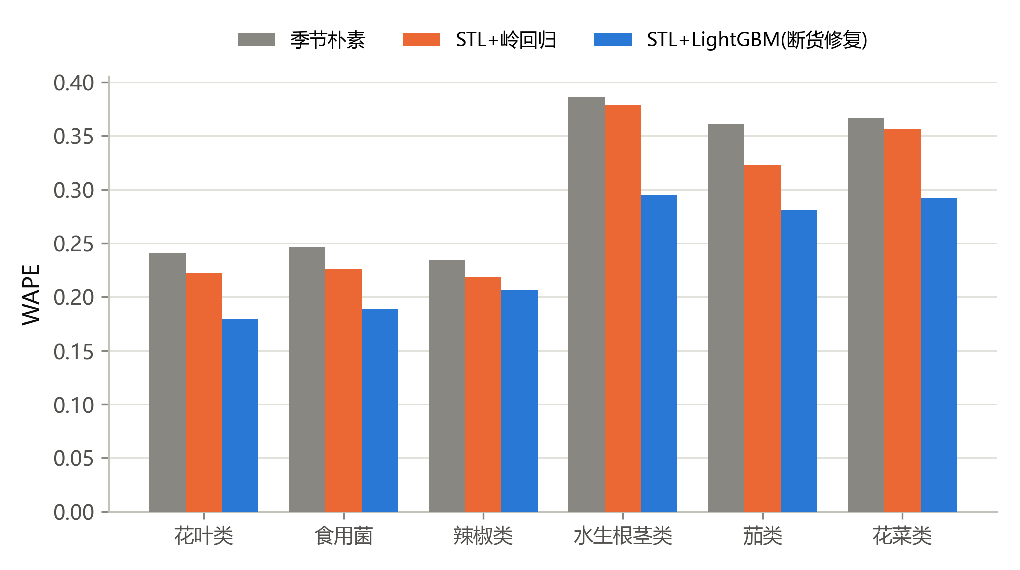
\includegraphics[width=0.92\textwidth]{paper_fig5.pdf}
  \caption{分品类 WAPE 对照:主模型与两条基线(24 折滚动平均)}
  \label{fig:wape}
\end{figure}

\subsubsection{七日需求量预测结果}

按消融结论,最终模型采用断货修复处理、以全部历史重训,输出 2023 年 7 月 1 日至 7 日六品类的日需求量 P10、P50、P90。表 \ref{tab:fc} 给出 P50 中位预测。

\begin{table}[htbp]
  \centering
  \caption{2023 年 7 月 1 日至 7 日六品类日需求量 P50 预测(kg/日)}
  \label{tab:fc}
  \begin{tabular}{lcccccc}
    \toprule
    日期 & 花叶类 & 食用菌 & 辣椒类 & 水生根茎类 & 茄类 & 花菜类 \\
    \midrule
    7 月 1 日 & 204.6 & 67.6 & 107.2 & 26.9 & 32.0 & 34.5 \\
    7 月 2 日 & 169.7 & 59.9 & 85.0 & 26.5 & 34.4 & 29.8 \\
    7 月 3 日 & 130.9 & 42.5 & 75.6 & 15.1 & 23.2 & 19.7 \\
    7 月 4 日 & 149.0 & 43.1 & 71.3 & 18.5 & 16.6 & 20.4 \\
    7 月 5 日 & 154.7 & 52.2 & 69.3 & 20.9 & 20.1 & 23.6 \\
    7 月 6 日 & 150.9 & 49.8 & 79.4 & 28.9 & 18.1 & 24.8 \\
    7 月 7 日 & 152.2 & 55.8 & 77.5 & 23.5 & 23.4 & 28.5 \\
    \bottomrule
  \end{tabular}
\end{table}

图 \ref{fig:fc} 以花叶类为例给出预测与近期历史的对照。7 月 1 日(周六)的预测为 204.6 kg,明显高于 6 月 30 日(周五)的 130.5 kg。本文对此作了专门核查:花叶类 6 月 30 日售满全天(最后成交时刻 21 时,与近 8 个同星期日的中位一致),未触发式 (\ref{eq:censor}) 的售罄标记,故就花叶类自身而言,该跳变不宜归因于断货,其来源是星期效应:花叶类近三年周六平均销量 229.3 kg,为全周最高,约为周一至周四均值的 1.4 倍,预测值恰好落在近期周六 161.5~244.3 kg 的区间之内。同时,预测窗前其他品类检出的提前售罄日(如花菜类 6 月 18 日)对应的被截断需求,已经由修复处理回补进训练目标,构成 7 月初需求水平上浮的次要因素。P10 至 P90 区间在周末与销量较大的品类上更宽,区间宽窄就是补货余量的选择空间:按 P50 补货,约半数日子会缺货;按 P90 补货,仅约一成日子缺货,但积压风险随之上升;两者如何取舍,交给第三问的收益模型结合缺货与损耗成本来确定。

\begin{figure}[H]
  \centering
  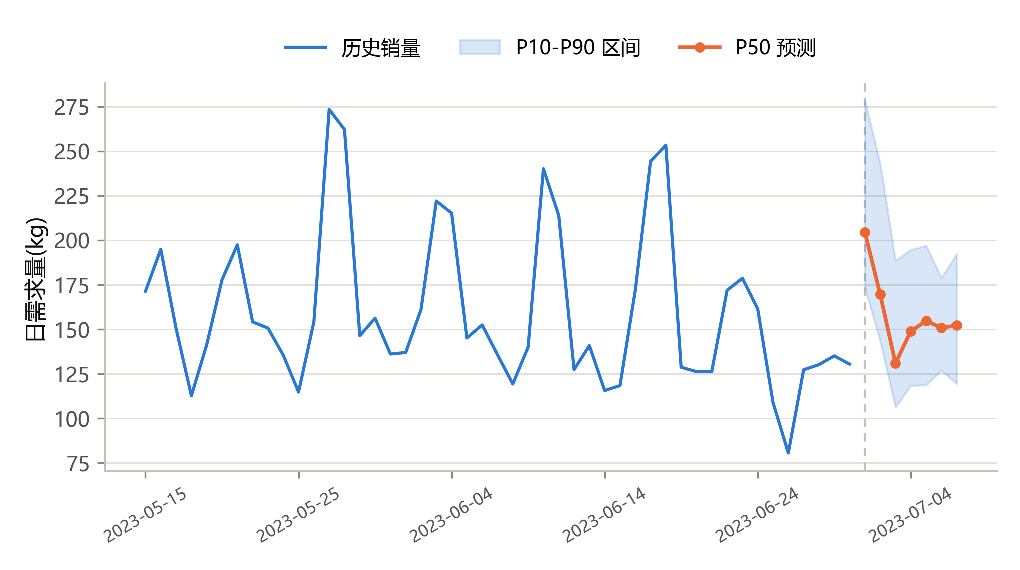
\includegraphics[width=0.92\textwidth]{paper_fig4.pdf}
  \caption{花叶类日需求量预测(2023 年 7 月 1 日至 7 日,近 45 天历史与 P10 至 P90 区间)}
  \label{fig:fc}
\end{figure}

\begin{thebibliography}{9}
% 并入小组主文档时,以下条目移入主文献表并统一编号
\bibitem{ke2017} Ke G, Meng Q, Finley T, et al. LightGBM: A highly efficient gradient boosting decision tree[C]//Advances in Neural Information Processing Systems 30. 2017: 3146-3154.
\bibitem{grinsztajn2022} Grinsztajn L, Oyallon E, Varoquaux G. Why do tree-based models still outperform deep learning on typical tabular data?[C]//Advances in Neural Information Processing Systems 35. 2022.
\bibitem{lyulyov2024} Lyulyov N N. The use of machine learning methods in demand forecasting in retail[C]//IFAC-PapersOnLine, 2024.
\bibitem{fan2024} Fan C L, Kuo C Y, Lu S Y, et al. Optimizing retail demand forecasting with LightGBM for rapid response supply chains[J]. Applied Sciences, 2024, 14(16): 7294.
\end{thebibliography}

%%FILL:AI使用声明占位(竞赛要求,参考文献前)%%
